
\begin{figure}
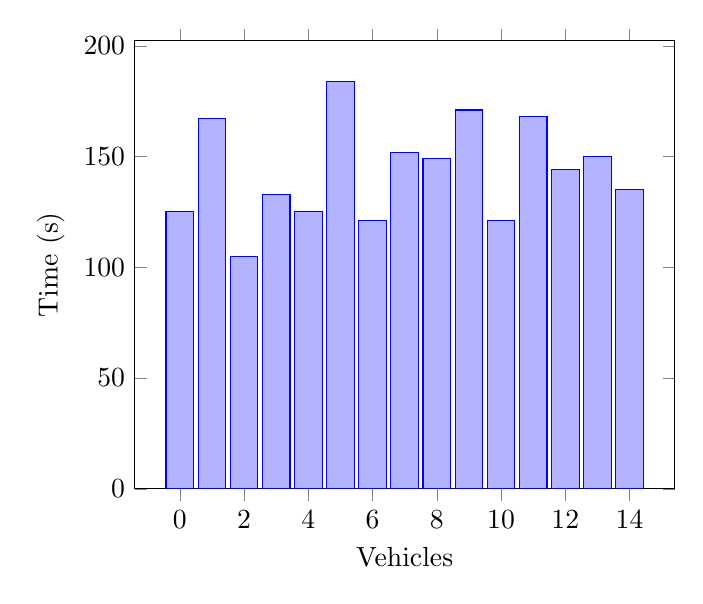
\begin{tikzpicture}
\begin{axis}[
legend style={anchor=west},
xlabel=Vehicles,
ylabel=Time (s),
ymin=0,
ybar,
]
\addplot coordinates {
(0, 125)
(1, 167)
(2, 105)
(3, 133)
(4, 125)
(5, 184)
(6, 121)
(7, 152)
(8, 149)
(9, 171)
(10, 121)
(11, 168)
(12, 144)
(13, 150)
(14, 135)
};

\end{axis}
\end{tikzpicture}
\label{tik:0:19_O, 19_O.-60, 17_N, 15_S, 15_S.-30, 13_N, 13_N.-40, 11_N, 8_N, 7_N, 7_N.-60, 5_N, 4_N, 4_N.-60, 2_V}
\caption{0 percent diving with GSC on route $19_O, 19_O.-60, 17_N, 15_S, 15_S.-30, 13_N, 13_N.-40, 11_N, 8_N, 7_N, 7_N.-60, 5_N, 4_N, 4_N.-60, 2_V$}
\end{figure}
